% =============================================================================
% Submissão à Revista Cadernos de Extensão (ISSN 2675-8164) — Edital 17/2026
% Centro Universitário do Distrito Federal — UDF
% =============================================================================
\documentclass[12pt,a4paper]{article}

\usepackage[utf8]{inputenc}
\usepackage[T1]{fontenc}
\usepackage[brazil]{babel}
\usepackage{times}
\usepackage[top=3cm,left=3cm,bottom=2cm,right=2cm]{geometry}
\usepackage{setspace}
\onehalfspacing
\usepackage{graphicx}
\usepackage{indentfirst}
\usepackage{booktabs}
\usepackage{caption}
\captionsetup{font={small,singlespacing},labelfont=bf,justification=centering}

% Citações em bloco: recuo de 1,25 cm e fonte menor (conforme edital)
\renewenvironment{quote}{%
  \begin{list}{}{%
    \setlength{\leftmargin}{1.25cm}%
    \setlength{\rightmargin}{0pt}%
    \setlength{\topsep}{6pt}%
  }\item[]\small\singlespacing%
}{\end{list}}
\usepackage{hyperref}
\hypersetup{colorlinks=true,linkcolor=black,citecolor=black,urlcolor=blue}
\usepackage[alf]{abntcite}
\bibliographystyle{abnt-alf}
% Macros usadas pelo .bbl que originalmente vêm de abntex2.cls
\providecommand{\abntrefinfo}[3]{}
\providecommand{\abntbstabout}[1]{}
\providecommand{\abntreprintinfo}[1]{\citeonline{#1}}

\setlength{\parindent}{1.25cm}
\setlength{\parskip}{0.2cm}

\title{\textbf{F\'abrica de Software Acad\^emica:\\
Relato da Experi\^encia no Centro Universit\'ario do Distrito Federal}}
\author{
  Esp.~Danrley Pereira\thanks{\texttt{danrley.pereira@cs.udf.edu.br}} \and
  Bel.~Rayssa Paiva \and
  Dra.~Let\'icia Zoby \and
  Dra.~Kerlla Luz\thanks{\texttt{kerlla.luz@udf.edu.br}} \\
  \small Centro Universit\'ario do Distrito Federal --- UDF \\
  \small Departamento de Engenharia, Arquitetura e TI
}
\date{2026}

\begin{document}
\maketitle

% =============================================================================
% RESUMO (até 250 palavras + 3-5 palavras-chave)
% =============================================================================
\section*{Resumo}
O presente relato de experi\^encia analisa o impacto da F\'abrica de
Software Acad\^emica do Centro Universit\'ario do Distrito Federal
(LabTech), entre 2022 e 2024, sobre o desenvolvimento de compet\^encias
t\'ecnicas e interpessoais de estudantes de TI, no \^ambito de uma a\c{c}\~ao
de extens\~ao universit\'aria. Adotou-se abordagem mista: dados
quantitativos dos reposit\'orios de c\'odigo (\emph{commits},
\emph{pull requests} e \emph{issues}) e do registro acad\^emico foram
triangulados com di\'arios de bordo, relat\'orios de est\'agio e observa\c{c}\~oes
em reuni\~oes. Adicionalmente, aplicou-se question\'ario estruturado a
quatorze participantes (n=14), composto pelo \emph{Entrepreneurship
Competence Framework} (EntreComp) da Comiss\~ao Europeia --- 17 itens em
escala de quatro pontos cobrindo autoconsci\^encia, mobiliza\c{c}\~ao de outros
e cria\c{c}\~ao de valor colaborativa --- e por uma adapta\c{c}\~ao de 20
itens da escala de autoefic\'acia de Sherer e colaboradores, em escala de
cinco pontos, com seis itens reversos recodificados. As respostas abertas foram analisadas pela t\'ecnica de
an\'alise de conte\'udo de Bardin. Os resultados indicam m\'edias elevadas
nas tr\^es dimens\~oes EntreComp (3,51; 3,54; 3,79 em escala 1--4) e
escores GSE concentrados na metade superior da escala (m\'edia=79,5;
faixa 67--90), convergindo com a evolu\c{c}\~ao observada em \emph{hard skills}
e \emph{soft skills}. A aus\^encia de protocolos padronizados de registro
foi reidentificada como principal limita\c{c}\~ao metodol\'ogica, parcialmente
endere\c{c}ada pelos instrumentos validados ora introduzidos. Conclui-se que
o modelo de F\'abrica de Software Acad\^emica \'e eficaz na aproxima\c{c}\~ao
entre teoria e pr\'atica, sendo a padroniza\c{c}\~ao instrumental caminho
promissor para mensura\c{c}\~ao longitudinal dos impactos formativos
extensionistas.

\noindent\textbf{Palavras-chave:} F\'abrica de Software Acad\^emica;
EntreComp; Autoefic\'acia; An\'alise de Conte\'udo; Extens\~ao Universit\'aria.

% =============================================================================
% ABSTRACT
% =============================================================================
\section*{Abstract}
\begin{otherlanguage*}{english}
This experience report analyses the impact of the Academic Software
Factory at Centro Universit\'ario do Distrito Federal (LabTech), between
2022 and 2024, on the development of technical and interpersonal
competences of IT students, within a university extension initiative. A
mixed-methods approach was adopted: quantitative data from code
repositories (commits, pull requests and issues) and academic records
were triangulated with project diaries, internship reports and meeting
observations. In addition, a structured questionnaire was administered
to fourteen participants (n=14), comprising the European Commission's
Entrepreneurship Competence Framework (EntreComp) --- 17 four-point items
covering self-awareness, mobilising others and collaborative value
creation --- and a 20-item adaptation of Sherer et al.'s Self-Efficacy
Scale, on a five-point scale, with six reverse items recoded. Open-ended answers
were processed through Bardin's content analysis. Results show high mean
scores across all EntreComp dimensions (3.51; 3.54; 3.79 on a 1--4
scale) and self-efficacy scores concentrated in the upper half of the
scale (mean=79.5; range 67--90), converging with the observed
development of hard and soft skills. The lack of standardised recording
protocols was reaffirmed as the main methodological limitation, although
partially addressed by the validated instruments introduced here. The
Academic Software Factory model proves effective in bridging theory and
practice, with instrument standardisation emerging as a promising path
for longitudinal measurement of extensionist training outcomes.

\vspace{\baselineskip}\noindent
\textbf{Keywords}: Academic Software Factory; EntreComp; Self-Efficacy;
Content Analysis; University Extension.
\end{otherlanguage*}

\newpage

% =============================================================================
% 1 INTRODUÇÃO
% =============================================================================
\section{Introdu\c{c}\~ao}
\label{sec:introducao}

O setor de Tecnologia da Informa\c{c}\~ao (TI) tem desempenhado papel cada
vez mais relevante no desenvolvimento econ\^omico e social do pa\'is.
Segundo a Empresa Brasil de Comunica\c{c}\~ao, com base em estudo da
FecomercioSP, registrou-se crescimento de 95\% de empregos ligados \`a
\'area de tecnologia na \'ultima d\'ecada \cite{ebctecnologia2024},
especialmente em polos emergentes como Bras\'ilia, que abriga
institui\c{c}\~oes p\'ublicas, privadas e centros de pesquisa, e cuja
economia \'e majoritariamente baseada em servi\c{c}os
($\sim$95\% do PIB local), configurando ambiente prop\'icio \`a demanda
por solu\c{c}\~oes digitais \cite{agenciapib2020}.

A conjuntura mundial de transforma\c{c}\~ao do trabalho refor\c{c}a essa
demanda. O \emph{Future of Jobs Report 2025}, do F\'orum Econ\^omico
Mundial \cite{wef:2025}, projeta que pensamento anal\'\i tico, lideran\c{c}a
e influ\^encia social, aprendizagem cont\'\i nua e alfabetiza\c{c}\~ao
tecnol\'ogica figuram entre as habilidades mais demandadas at\'e 2030 ---
combinando, portanto, \emph{hard skills} t\'ecnicas e \emph{soft skills}
comportamentais. Nesse contexto, a cria\c{c}\~ao de uma F\'abrica de
Software em ambiente acad\^emico --- conceito originalmente cunhado por
\citeonline{cusumano1991japan} para descrever a sistematiza\c{c}\~ao do
desenvolvimento de \emph{software} no modelo industrial japon\^es ---
surge como oportunidade estrat\'egica para integrar teoria e pr\'atica,
preparando os estudantes para os desafios reais do mercado e
desenvolvendo solu\c{c}\~oes voltadas \`as demandas da sociedade
\cite{bernardi2017learning,oliveira2017conduccao}.

Como a\c{c}\~ao de extens\~ao universit\'aria, o projeto LabTech do Centro
Universit\'ario do Distrito Federal (UDF) cumpre dupla fun\c{c}\~ao: amplia
a forma\c{c}\~ao discente para al\'em da sala de aula
\cite{santos2021experiencia} e socializa com a comunidade os produtos da
pesquisa e do ensino. Por meio de projetos orientados por metodologias
\'ageis, ferramentas contempor\^aneas e acompanhamento de mentores,
desenvolvem-se compet\^encias t\'ecnicas (\emph{hard skills}) e
interpessoais (\emph{soft skills}), como comunica\c{c}\~ao, trabalho em
equipe e lideran\c{c}a \cite{perides2021competencias}. O presente artigo
relata a experi\^encia de implanta\c{c}\~ao e consolida\c{c}\~ao deste modelo
no UDF, destaca os benef\'icios para a forma\c{c}\~ao discente, discute as
boas pr\'aticas adotadas e os desafios enfrentados, e introduz, de forma
in\'edita no projeto, instrumentos validados de mensura\c{c}\~ao de
compet\^encias --- o \emph{Entrepreneurship Competence Framework}
(EntreComp) da Comiss\~ao Europeia \cite{bacigalupo2016entrecomp} e a
\emph{General Self-Efficacy Scale} (GSE) de \citeonline{sherer1982gse}.

Conforme \citeonline[p.~15]{ander-egg1978}, ``a Ci\^encia \'e um conjunto
de conhecimentos racionais, certos ou prov\'aveis, obtidos metodicamente,
sistematizados e verific\'aveis, que fazem refer\^encia a objetos de uma
mesma natureza''. Esse enfoque justifica a ado\c{c}\~ao de m\'etodos e
t\'ecnicas que aux\'iliem na padroniza\c{c}\~ao dos processos e na an\'alise
cr\'itica dos resultados em uma F\'abrica de Software Acad\^emica,
motiva\c{c}\~ao central deste estudo.

O artigo est\'a estruturado em cinco se\c{c}\~oes principais ap\'os esta
introdu\c{c}\~ao: a Se\c{c}\~ao~\ref{sec:metodologia} descreve a metodologia,
incluindo o l\'ocus da pesquisa, os procedimentos do LabTech e os
instrumentos adotados; a Se\c{c}\~ao~\ref{sec:resultados} apresenta os
resultados, com o perfil dos participantes, m\'etricas dos reposit\'orios
e os escores nos instrumentos EntreComp e GSE; a
Se\c{c}\~ao~\ref{sec:analise-discussao} discute os achados \`a luz da
literatura e dos di\'arios de bordo; a Se\c{c}\~ao~\ref{sec:conclusao}
apresenta as conclus\~oes e as agendas de trabalhos futuros.

% =============================================================================
% 2 METODOLOGIA
% =============================================================================
\section{Metodologia}
\label{sec:metodologia}

Trata-se de um estudo descritivo do tipo relato de experi\^encia, de
natureza qualitativa-quantitativa, sobre a implementa\c{c}\~ao e a
gest\~ao da F\'abrica de Software Acad\^emica LabTech no UDF, no per\'iodo
2022--2024.

\subsection{L\'ocus da Pesquisa}
\label{sec:locus}

O Centro Universit\'ario do Distrito Federal (UDF), fundado em 1967,
destaca-se como uma das pioneiras no ensino superior particular em
Bras\'ilia. Com cursos em diversas \'areas, promove ensino, pesquisa e
extens\~ao na regi\~ao \cite{udfppc2023}. O Departamento de Engenharia,
Arquitetura e TI abrange os cursos de An\'alise e Desenvolvimento de
Sistemas (ADS), Ci\^encia da Computa\c{c}\~ao (CCP), Sistemas de
Informa\c{c}\~ao (SI), Design Gr\'afico (DG) e Engenharia de Software
(ENG), todos enquadrados nas Diretrizes Curriculares Nacionais para a
\'area da Computa\c{c}\~ao \cite{dcncomputacao2016}.
Nos \'ultimos dois anos observou-se crescimento expressivo nas
matr\'iculas (Tabela~\ref{tab:matriculas-ti}).

\begin{table}[ht]
\centering
\small
\caption{Evolu\c{c}\~ao das matr\'iculas nos cursos de TI (2022--2024). Fonte: sistema interno da UDF.}
\label{tab:matriculas-ti}
\begin{tabular}{lrrr}
\hline
\textbf{Curso} & \textbf{2022} & \textbf{2023} & \textbf{2024*} \\
\hline
Engenharia de Software & n/a & n/a & 123 \\
Ci\^encia da Computa\c{c}\~ao & 380 & 520 & 639 \\
Sistemas de Informa\c{c}\~ao & 300 & 400 & 148 \\
Design Gr\'afico & 200 & 270 & 201 \\
An\'alise e Desenvolvimento de Sistemas & 150 & 160 & 696 \\
\hline
\textbf{Total} & \textbf{1.530} & \textbf{2.000} & \textbf{1.807} \\
\hline
\multicolumn{4}{l}{\footnotesize * Dados consolidados de 2025.}
\end{tabular}
\end{table}

\subsection{Procedimentos do LabTech}
\label{sec:procedimentos}

A organiza\c{c}\~ao do LabTech segue a defini\c{c}\~ao cl\'assica de
F\'abrica de Software como processo estruturado, controlado e
continuamente aprimorado para o desenvolvimento de \emph{software}
\cite{fernandes2004fabrica}, transposta para o contexto acad\^emico.
As equipes s\~ao organizadas de forma multidisciplinar, com
pap\'eis adapt\'aveis (desenvolvedor, gerente de projetos, analista de
dados, designer de interface, analista de seguran\c{c}a) e reuni\~oes
peri\'odicas para planejar e revisar as atividades. Ferramentas como
GitHub, Trello, Jira, Discord e Figma sustentam as cerim\^onias do
\emph{framework} SCRUM e o controle de demandas via quadros KANBAN.
Em alguns projetos utilizam-se tecnologias como Spring Boot, Flask e
React, permitindo o contato com \emph{frameworks} contempor\^aneos. Os
projetos em desenvolvimento incluem o Sistema de Reserva de Salas, o
Sistema de Eventos e o Sistema de Aloca\c{c}\~ao de Professores; a
arquitetura est\'a ilustrada na Figura~\ref{fig:topologia}.

\begin{figure}[h!]
    \centering
    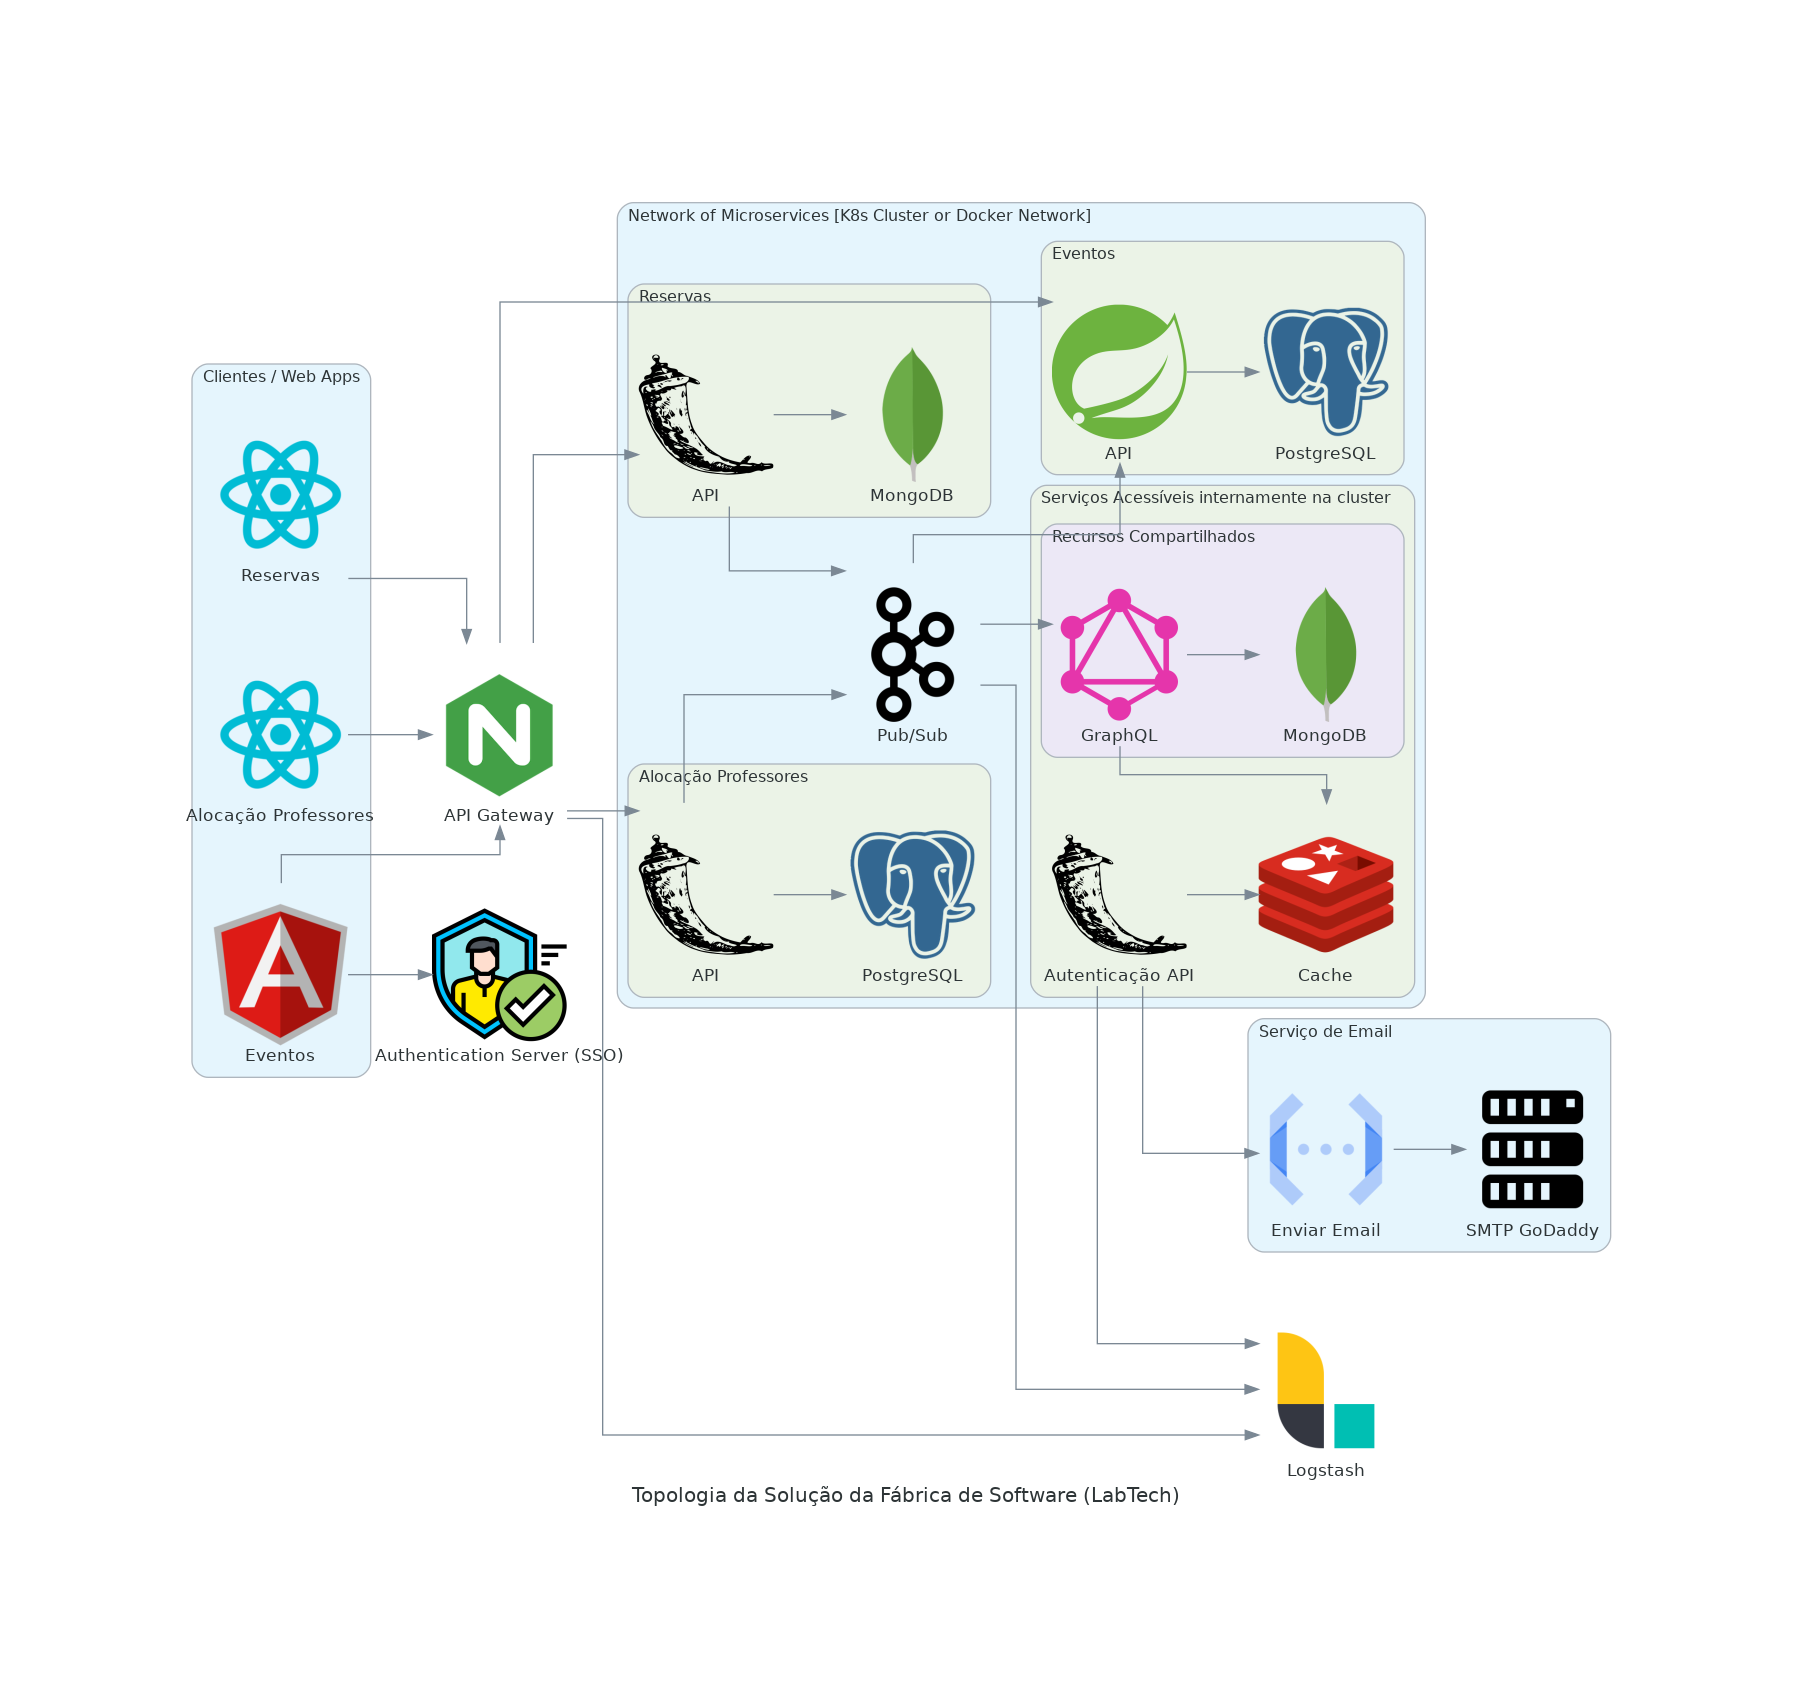
\includegraphics[width=0.8\textwidth]{topologia.png}
    \caption{Topologia da solu\c{c}\~ao do LabTech/UDF.}
    \label{fig:topologia}
\end{figure}

\subsection{Abordagem Qualitativa e Quantitativa}
\label{sec:abordagem}

Optou-se por estrat\'egia mista para capturar tanto elementos num\'ericos
quanto interpretativos da din\^amica do LabTech. As fontes quantitativas
incluem matr\'iculas, frequ\^encia de participa\c{c}\~ao e atividade nos
reposit\'orios (\emph{commits}, \emph{pull requests}, \emph{issues}). As
fontes qualitativas compreendem di\'arios de bordo dos alunos-gerentes,
relat\'orios semanais e finais, e observa\c{c}\~oes diretas em reuni\~oes,
revis\~oes de c\'odigo e an\'alise de \emph{issues} --- procedimentos
inspirados na tradi\c{c}\~ao etnogr\'afica aplicada \`a educa\c{c}\~ao,
que privilegia a observa\c{c}\~ao prolongada e situada das pr\'aticas
cotidianas dos sujeitos investigados \cite{mattos2011etnografia}. Os dados foram
\emph{triangulados} considerando tr\^es dimens\~oes: t\'ecnica
(tecnologias, padr\~oes de projeto), gerencial (organiza\c{c}\~ao do
\emph{backlog}, comunica\c{c}\~ao) e educacional (desenvolvimento de
\emph{hard} e \emph{soft skills}).

\subsection{Instrumentos de Coleta de Compet\^encias}
\label{sec:instrumentos}

Em fevereiro de 2025 aplicou-se question\'ario estruturado aos
participantes do LabTech ($n=14$), integrando dois invent\'arios
consagrados na literatura. O primeiro, com 17 itens em escala Likert de
quatro pontos (1 -- Discordo Totalmente; 4 -- Concordo Totalmente),
deriva do \emph{Entrepreneurship Competence Framework} (EntreComp),
proposto pela Comiss\~ao Europeia \cite{bacigalupo2016entrecomp},
organizado em tr\^es dimens\~oes: autoconsci\^encia e autoefic\'acia
(itens 1--6, \'area \emph{Ideias e Oportunidades}); mobiliza\c{c}\~ao de
outros (itens 7--11, \'area \emph{Recursos})\footnote{Os itens 9 e 11 do
question\'ario aplicado apresentam enunciado id\^entico (``Eu posso
mostrar empatia para com os outros.''), artefato do instrumento de
coleta. Optou-se por mant\^e-los na an\'alise para preservar a integridade
dos dados, com ci\^encia de leve infla\c{c}\~ao poss\'ivel na m\'edia desta
dimens\~ao.}; e cria\c{c}\~ao de valor colaborativa (itens 12--17, \'area
\emph{Em A\c{c}\~ao}). O segundo \'e uma adapta\c{c}\~ao de 20 itens, em
escala de cinco pontos, da escala de autoefic\'acia originalmente proposta
por \citeonline{sherer1982gse} \emph{Self-Efficacy Scale}\footnote{A
escala original de Sherer e colaboradores (1982) cont\'em 23 itens
distribu\'\i dos em duas dimens\~oes: 17 itens de autoefic\'acia geral e 6
itens de autoefic\'acia social. A vers\~ao de 20 itens utilizada neste
estudo segue adapta\c{c}\~oes posteriores publicadas em pesquisas
internacionais voltadas para autoefic\'acia em contextos profissionais e
acad\^emicos.}; os itens 8, 11, 13, 16, 18 e 20 s\~ao formulados de modo
invertido e foram recodificados como $6-x$ antes da an\'alise, de modo a
fazer com que todos os itens apontem na mesma dire\c{c}\~ao
(maior = maior autoefic\'acia percebida).

As respostas abertas foram tratadas pela t\'ecnica de an\'alise de
conte\'udo de \citeonline{bardin2011}, organizada em tr\^es fases:
pr\'e-an\'alise (leitura flutuante e identifica\c{c}\~ao de unidades de
sentido), explora\c{c}\~ao do material (codifica\c{c}\~ao tem\'atica em
categorias-semente) e tratamento dos resultados (interpreta\c{c}\~ao em
di\'alogo com os achados quantitativos). A codifica\c{c}\~ao foi
operacionalizada por busca de express\~oes regulares sobre os trechos,
com revis\~ao manual.

\subsection{Limita\c{c}\~oes Metodol\'ogicas}
\label{sec:limitacoes}

A principal limita\c{c}\~ao reside na \textbf{aus\^encia de um protocolo
\'unico de registro} --- incluindo di\'arios de bordo e atas de reuni\~ao
sistematizados --- que compromete a realiza\c{c}\~ao de an\'alises
comparativas mais rigorosas \cite{mineiro2022pesquisa}. Em cada equipe,
a ado\c{c}\~ao de ferramentas e processos segue prefer\^encias aut\^onomas,
reduzindo a uniformidade dos dados. Ademais, a inexist\^encia de um
\emph{software} em produ\c{c}\~ao efetiva dificulta a an\'alise de
m\'etricas relacionadas \`a satisfa\c{c}\~ao ou \`a ado\c{c}\~ao pelos
usu\'arios. A amostra do question\'ario ($n=14$) e o intervalo
temporal (2022--2024) reposicionam os achados como evid\^encias
explorat\'orias, n\~ao inferenciais.

% =============================================================================
% 3 RESULTADOS
% =============================================================================
\section{Resultados}
\label{sec:resultados}

\subsection{Perfil dos Participantes}
\label{sec:perfil}

Os participantes do LabTech distribuem-se entre os cursos de Ci\^encia
da Computa\c{c}\~ao (CCP), Sistemas de Informa\c{c}\~ao (SI) e An\'alise e
Desenvolvimento de Sistemas (ADS), com diferentes formas de v\'inculo
(est\'agio supervisionado, monitoria para horas complementares, convite
da coordena\c{c}\~ao e trabalho volunt\'ario). As Figuras
\ref{fig:distribuicao_semestre} a \ref{fig:participacao_ano} sintetizam
a distribui\c{c}\~ao por semestre, a classifica\c{c}\~ao de experi\^encia
pr\'evia, as tecnologias mais citadas, o n\'umero de estudantes por curso
e a participa\c{c}\~ao por ano.

\begin{figure}[!htbp]
    \centering
    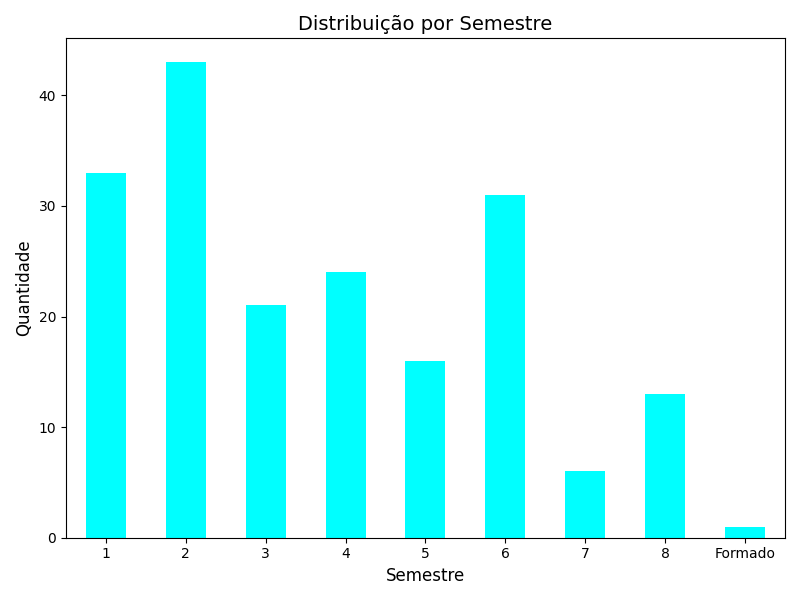
\includegraphics[width=0.55\textwidth]{assets/perfil/distribuicao_por_semestre.png}
    \caption{Distribui\c{c}\~ao dos participantes por semestre.}
    \label{fig:distribuicao_semestre}
\end{figure}

\begin{figure}[!htbp]
    \centering
    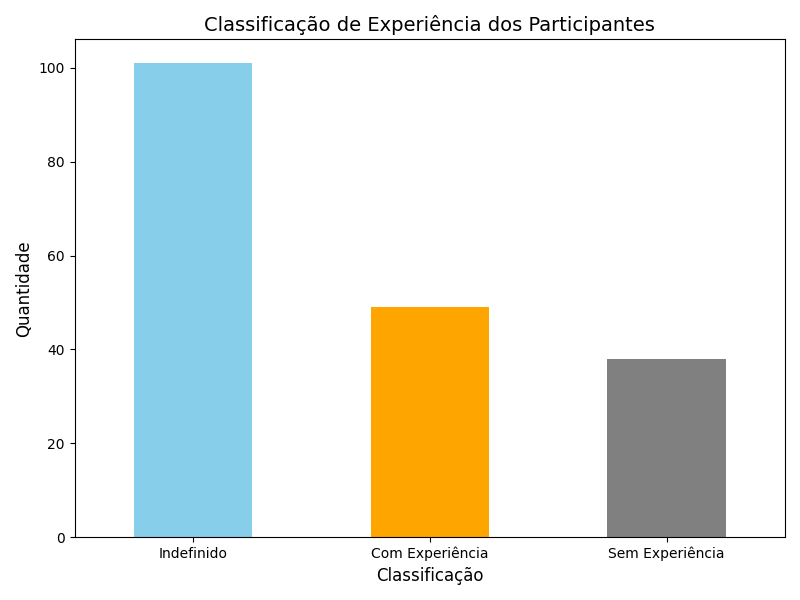
\includegraphics[width=0.55\textwidth]{assets/perfil/experiencia_classificacao.png}
    \caption{Classifica\c{c}\~ao de experi\^encia dos participantes.}
    \label{fig:experiencia_classificacao}
\end{figure}

\begin{figure}[!htbp]
    \centering
    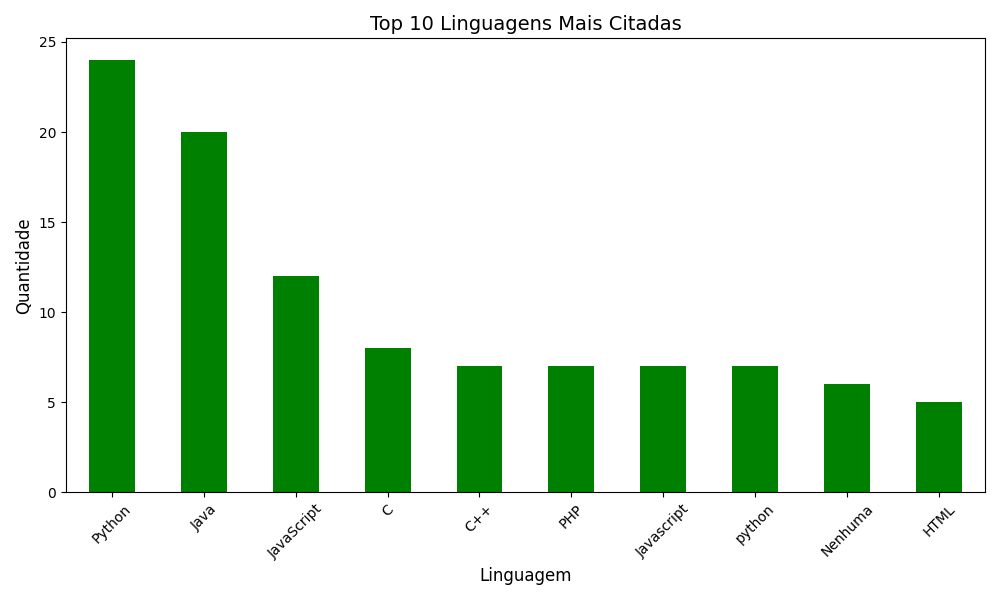
\includegraphics[width=0.75\textwidth]{assets/perfil/top_linguagens_citadas.png}
    \caption{As 10 linguagens mais citadas pelos participantes.}
    \label{fig:linguagens_citadas}
\end{figure}

\begin{figure}[!htbp]
    \centering
    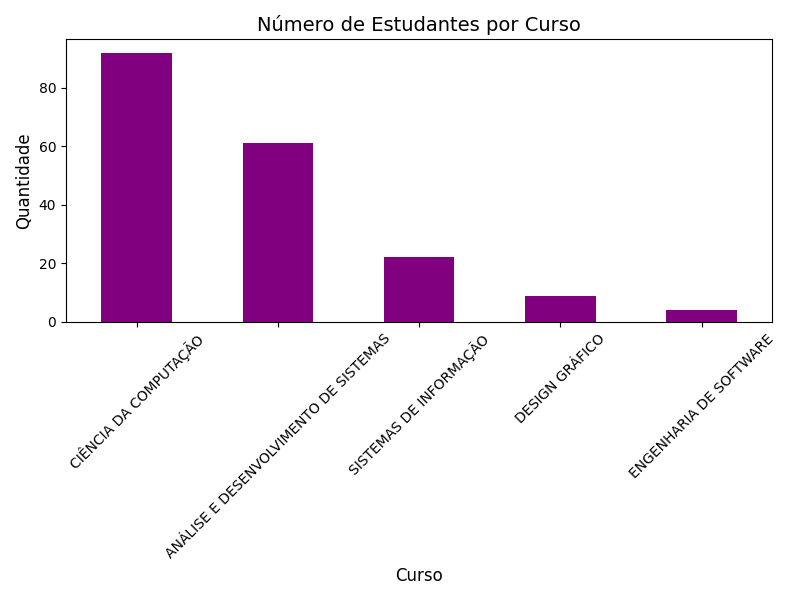
\includegraphics[width=0.65\textwidth]{assets/perfil/numero_estudantes_por_curso.png}
    \caption{N\'umero de estudantes por curso.}
    \label{fig:estudantes_curso}
\end{figure}

\begin{figure}[!htbp]
    \centering
    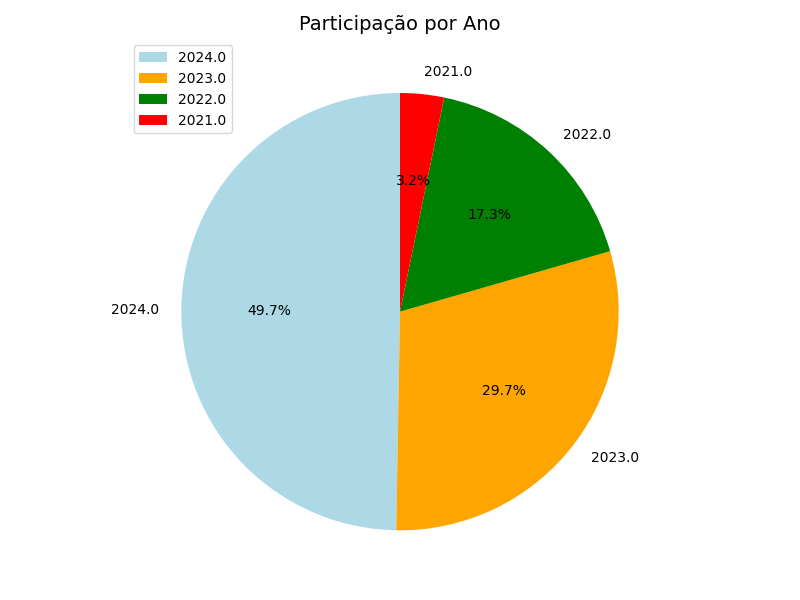
\includegraphics[width=0.65\textwidth]{assets/perfil/participacao_por_ano.png}
    \caption{Participa\c{c}\~ao por ano.}
    \label{fig:participacao_ano}
\end{figure}

\subsection{An\'alise dos Reposit\'orios}
\label{sec:repositorios}

A Figura~\ref{fig:heatmap_activity} apresenta um \emph{heatmap}
relacionando o dia da semana (eixo vertical) com a hora do dia (eixo
horizontal); a intensidade de cor representa o n\'umero de
contribui\c{c}\~oes (\emph{commits}, \emph{issues}, \emph{pull requests},
coment\'arios) em cada intervalo. Observa-se concentra\c{c}\~ao de
atividade em hor\'arios noturnos e no in\'icio da semana, possivelmente
decorrente da rotina acad\^emica e profissional dos participantes.

\begin{figure}[!htbp]
    \centering
    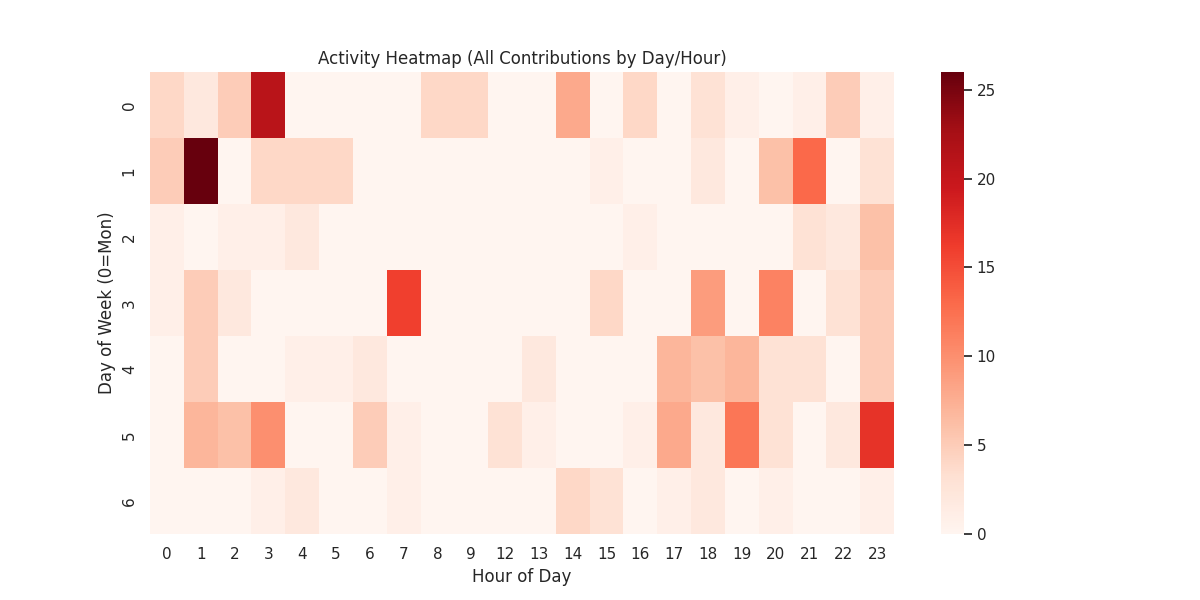
\includegraphics[width=0.65\textwidth]{assets/github/activity-heatmap.png}
    \caption{Heatmap de contribui\c{c}\~oes por dia/hora.}
    \label{fig:heatmap_activity}
\end{figure}

A Figura~\ref{fig:burndown} apresenta um \emph{burndown chart} que
evidencia a quantidade de \emph{issues} abertas ao longo do tempo, com
per\'iodos de estabilidade intercalados por picos coincidentes com o
in\'icio de novos \emph{sprints}.

\begin{figure}[!htbp]
    \centering
    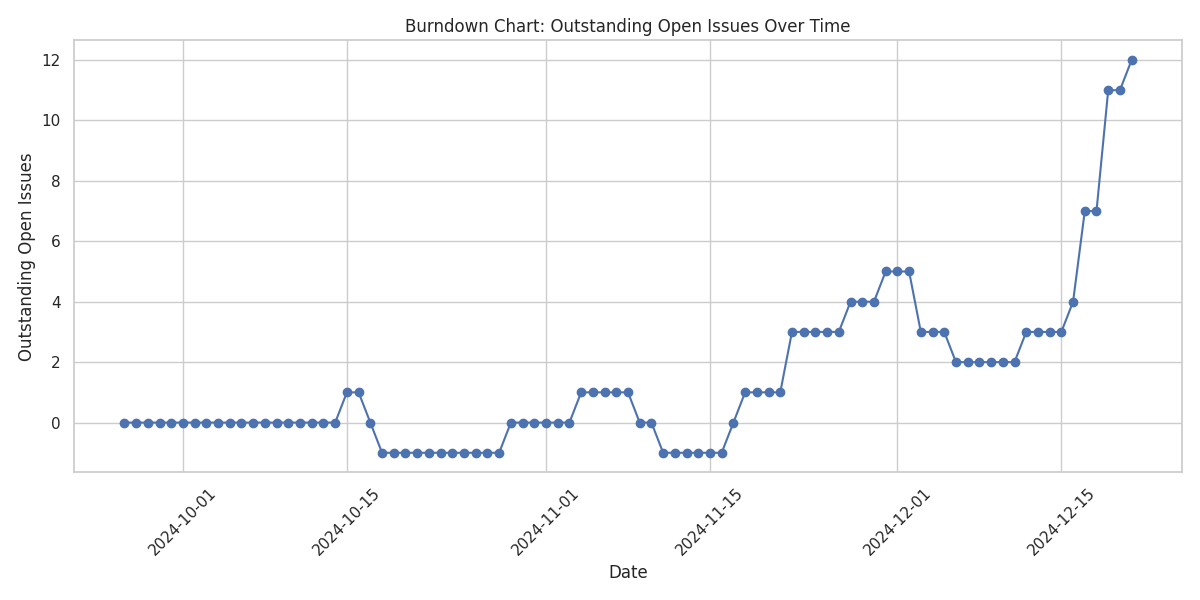
\includegraphics[width=0.65\textwidth]{assets/github/burndown-chart.png}
    \caption{\emph{Burndown chart}: \emph{issues} pendentes ao longo do tempo.}
    \label{fig:burndown}
\end{figure}

A rede de colabora\c{c}\~ao (Figura~\ref{fig:rede}) mostra n\'os
correspondentes a cada membro e arestas representando a co-participa\c{c}\~ao
em reposit\'orios e \emph{issues}. A distribui\c{c}\~ao de \emph{commits}
por membro \'e ilustrada pelo \emph{box plot}
(Figura~\ref{fig:commit_box}); observa-se que alguns participantes
realizam um elevado n\'umero de \emph{commits}, enquanto outros
apresentam atividade m\'inima.

\begin{figure}[!htbp]
    \centering
    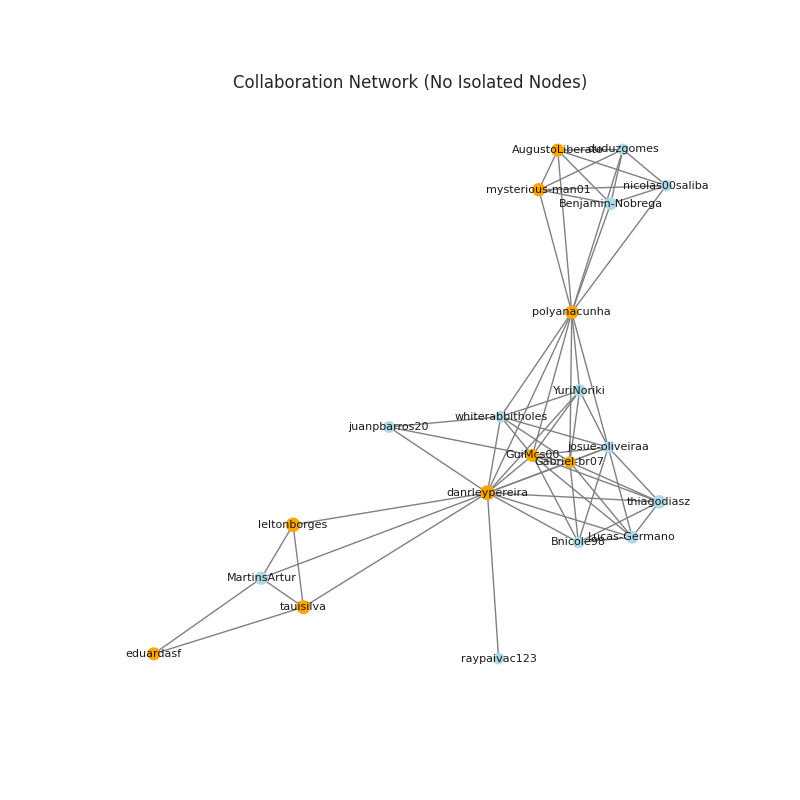
\includegraphics[width=0.6\textwidth]{assets/github/collaboration-network-no-isolated.png}
    \caption{Rede de colabora\c{c}\~ao (excluindo n\'os isolados).}
    \label{fig:rede}
\end{figure}

\begin{figure}[!htbp]
    \centering
    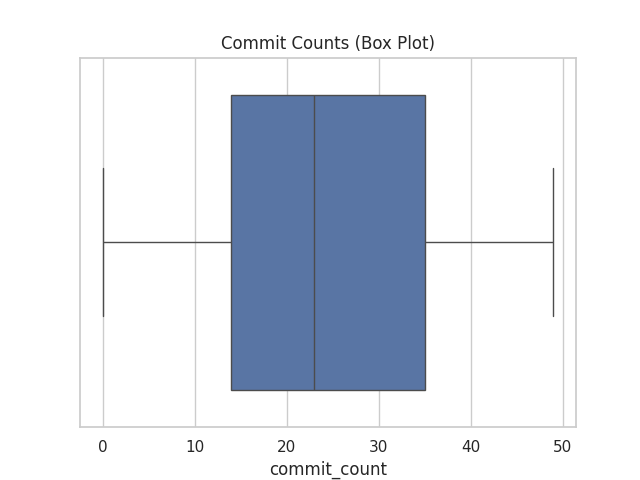
\includegraphics[width=0.55\textwidth]{assets/github/commit-boxplot.png}
    \caption{Distribui\c{c}\~ao de \emph{commits} por membro.}
    \label{fig:commit_box}
\end{figure}

\subsection{Compet\^encias Autorrelatadas: EntreComp e Autoefic\'acia}
\label{sec:resultados-survey}

A aplica\c{c}\~ao dos instrumentos descritos na
Se\c{c}\~ao~\ref{sec:instrumentos} obteve 14 respostas v\'alidas, de
participantes vinculados ao LabTech entre 2022 e 2024 nos cursos de CCP,
SI e ADS. A Figura~\ref{fig:entrecomp_dimensoes} sintetiza as m\'edias
por dimens\~ao EntreComp (escala 1--4); a
Figura~\ref{fig:entrecomp_distribuicao} apresenta a distribui\c{c}\~ao
Likert por item; a Tabela~\ref{tab:competencias-resumo} resume m\'edias e
desvios.

\begin{figure}[!htbp]
    \centering
    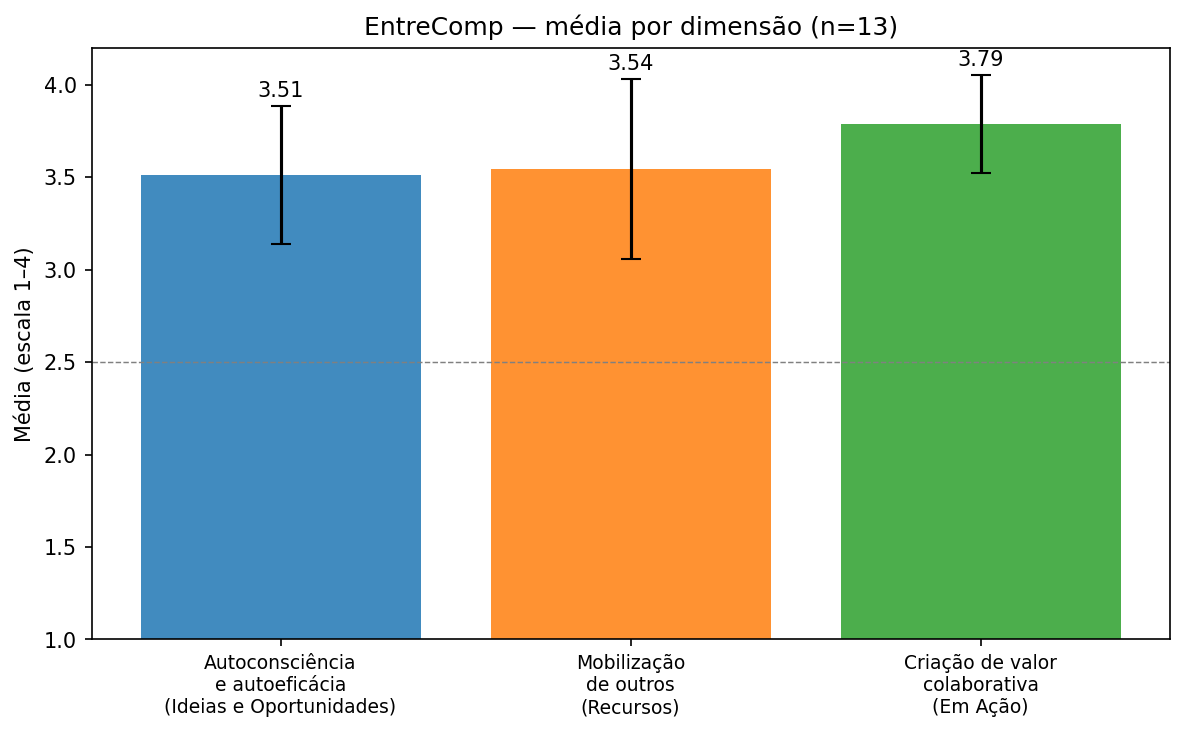
\includegraphics[width=0.7\textwidth]{assets/competencias/graficos/entrecomp_means_por_dimensao.png}
    \caption{M\'edias por dimens\~ao EntreComp (n=14).}
    \label{fig:entrecomp_dimensoes}
\end{figure}

\begin{figure}[!htbp]
    \centering
    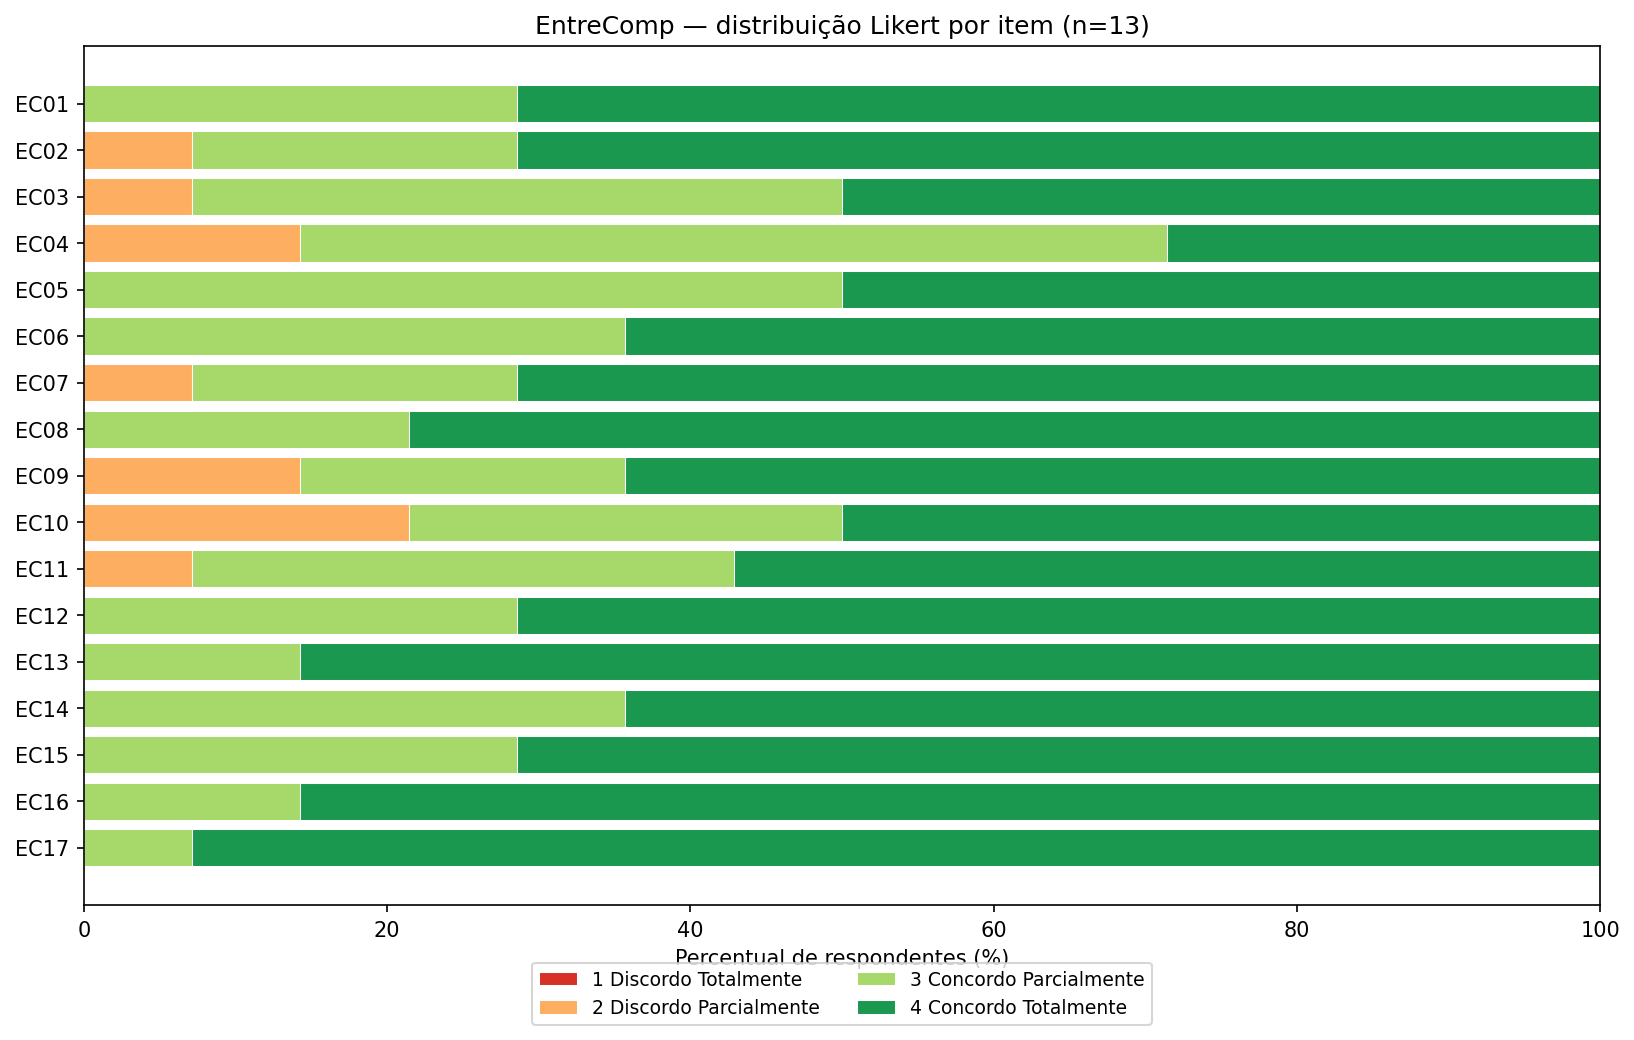
\includegraphics[width=0.85\textwidth]{assets/competencias/graficos/entrecomp_distribuicao_likert.png}
    \caption{Distribui\c{c}\~ao Likert por item EntreComp (n=14).}
    \label{fig:entrecomp_distribuicao}
\end{figure}

\begin{table}[!htbp]
\centering
\caption{Resumo descritivo das dimensões EntreComp e GSE (n=14).}
\label{tab:competencias-resumo}
\small
\begin{tabular}{lccccc}
\hline
\textbf{Dimensão} & \textbf{Itens} & \textbf{Média} & \textbf{Desvio} & \textbf{Mín.} & \textbf{Máx.} \\
\hline
Autoconsciência e autoeficácia (Ideias e Oportunidades) & 6 & 3.51 & 0.37 & 2.83 & 4.00 \\
Mobilização de outros (Recursos) & 5 & 3.54 & 0.49 & 2.60 & 4.00 \\
Criação de valor colaborativa (Em Ação) & 6 & 3.79 & 0.27 & 3.17 & 4.00 \\
GSE -- escore total (1–5 por item, agregado) & 20 & 3.98 & 0.33 & 3.35 & 4.50 \\
GSE -- escore total (faixa 20–100) & 20 & 79.50 & 6.65 & 67.00 & 90.00 \\
\hline
\end{tabular}
\end{table}


Observa-se predomin\^ancia de escores pr\'oximos ao limite superior nas
tr\^es dimens\~oes EntreComp, com destaque para \emph{cria\c{c}\~ao de
valor colaborativa} (m\'edia=3,79; $\sigma$=0,27), seguida por
\emph{mobiliza\c{c}\~ao de outros} (3,54) e \emph{autoconsci\^encia e
autoefic\'acia} (3,51).

No instrumento GSE \cite{sherer1982gse}, ap\'os a invers\~ao dos itens
8, 11, 13, 16, 18 e 20, o escore total (faixa te\'orica 20--100)
apresentou m\'edia=79,5 e desvio=6,65, com m\'inimo de 67 e m\'aximo de 90,
distribui\c{c}\~ao concentrada na metade superior da escala
(Figura~\ref{fig:gse_total}). Este padr\~ao sugere n\'ivel elevado de
autoefic\'acia percebida entre os respondentes.

\begin{figure}[!htbp]
    \centering
    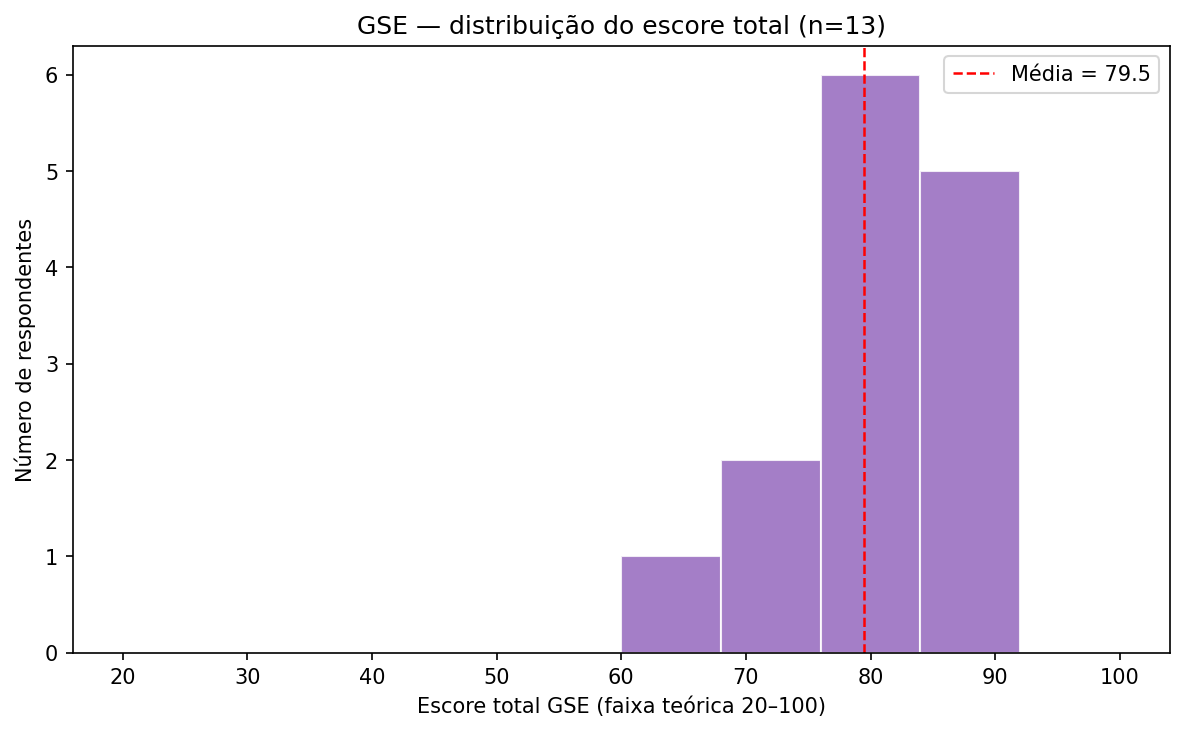
\includegraphics[width=0.65\textwidth]{assets/competencias/graficos/gse_total_distribuicao.png}
    \caption{Distribui\c{c}\~ao do escore total da GSE (n=14).}
    \label{fig:gse_total}
\end{figure}

A an\'alise de conte\'udo \cite{bardin2011} das seis respostas abertas
v\'alidas evidenciou tr\^es categorias recorrentes: \emph{ganho de
autonomia t\'ecnica} (4 men\c{c}\~oes), \emph{diversidade de perspectivas}
(2) e \emph{sustentabilidade externa do programa} (2). Trechos
ilustrativos:

\begin{quote}\small
``Deu muito pra mim ter trocas de conhecimentos e conhecer colegas de
outros cursos, agregando para o projeto diferentes perspectivas''
(R01, CCP, 23 anos).
\end{quote}

\begin{quote}\small
``Foi uma excelente oportunidade para conhecer as diversas \'areas de
atua\c{c}\~ao dentro de um projeto de desenvolvimento, al\'em de
proporcionar uma imers\~ao completa no processo de cria\c{c}\~ao de um
sistema, desde o planejamento at\'e a entrega'' (R02, SI, 28 anos).
\end{quote}

\begin{quote}\small
``Uma completa falta de organiza\c{c}\~ao e did\'atica, especialmente para
quem tava come\c{c}ando a programar'' (R05, CCP, 21 anos).
\end{quote}

% =============================================================================
% 4 ANÁLISE E DISCUSSÃO
% =============================================================================
\section{An\'alise e Discuss\~ao}
\label{sec:analise-discussao}

\subsection{Aspectos T\'ecnicos}
Os registros dos di\'arios de bordo indicam que a ado\c{c}\~ao de
\emph{frameworks} modernos (Spring Boot, Flask, React) contribuiu para
o aprimoramento das compet\^encias t\'ecnicas. Desafios como
configura\c{c}\~ao de ambientes, controle de vers\~ao e integra\c{c}\~ao
cont\'inua foram recorrentes, exigindo suporte cont\'inuo dos
orientadores e dos alunos-gerentes; tais dificuldades, contudo,
representaram oportunidades de aprendizagem que fortaleceram a
autonomia t\'ecnica dos estudantes --- categoria expressivamente
destacada na an\'alise de conte\'udo (66,7\% das respostas abertas
v\'alidas).

\subsection{Aspectos Gerenciais}
A aus\^encia de pap\'eis formais (\emph{Scrum Master}, \emph{Product
Owner}) imp\^os maior autonomia aos alunos-gerentes, sobretudo na
media\c{c}\~ao de conflitos e na organiza\c{c}\~ao do \emph{backlog}.
Problemas de comunica\c{c}\~ao ocorreram, principalmente, quando
indisponibilidades n\~ao eram informadas tempestivamente. Reuni\~oes
semanais e revis\~oes de c\'odigo (\emph{code reviews}) mitigaram esses
problemas. A aus\^encia de relat\'orios padronizados, no entanto,
dificultou a identifica\c{c}\~ao precoce de gargalos --- ponto refor\c{c}ado
pela cr\'itica direta de R05 quanto \`a ``falta de organiza\c{c}\~ao e
did\'atica''.

\subsection{Aspectos Educacionais}
As m\'edias EntreComp elevadas (3,51--3,79 em escala 1--4) e os escores
GSE concentrados na metade superior da escala (m\'edia=79,5/100)
convergem com os relatos qualitativos de melhoria em autoconfian\c{c}a,
trabalho em equipe e tomada de decis\~ao sob press\~ao. A maior pontua\c{c}\~ao
\textbf{na dimens\~ao de cria\c{c}\~ao colaborativa de valor} (3,79)
\'e consistente com o car\'ater extensionista do LabTech, no qual o
estudante interage continuamente com pares de cursos distintos para
entregar artefatos de software \'uteis ao ambiente acad\^emico ---
categoria \emph{diversidade de perspectivas} corroborada por R01 e R02.

A pr\'opria sele\c{c}\~ao da amostra precisa ser considerada na
interpreta\c{c}\~ao: respondentes vinculados ao LabTech tendem a apresentar
maior engajamento e autoconfian\c{c}a, o que pode contribuir para os
escores elevados observados. A aus\^encia de uma medi\c{c}\~ao
pr\'e-LabTech impede inferir causalidade direta; contudo, a converg\^encia
entre dados quantitativos (instrumentos validados) e qualitativos
(an\'alise de conte\'udo) refor\c{c}a a hip\'otese de que a
participa\c{c}\~ao no programa contribui para o desenvolvimento de
compet\^encias empreendedoras e de autoefic\'acia geral.

A formação extensionista propiciada pelo LabTech alinha-se ao perfil
delineado pelas Diretrizes Curriculares Nacionais para os cursos da
\'area da Computa\c{c}\~ao \cite{dcncomputacao2016}, que prescrevem o
desenvolvimento conjunto de compet\^encias t\'ecnicas e comportamentais
(comunica\c{c}\~ao, trabalho em equipe, capacidade de aprendizagem
cont\'\i nua). De forma similar, abordagens ativas de ensino-aprendizagem
em engenharia, como a perspectiva KAA descrita por
\citeonline{kerlla}, t\^em demonstrado que a imers\~ao em projetos reais
favorece simultaneamente a aquisi\c{c}\~ao de \emph{hard skills} e o
amadurecimento de \emph{soft skills} --- mecanismo coerente com os
escores observados nas tr\^es dimens\~oes EntreComp.

\subsection{Andaimagem Institucional (\emph{Scaffolding})}
\label{sec:scaffolding}

A cr\'\i tica direta de R05 (``uma completa falta de organiza\c{c}\~ao e
did\'atica, especialmente para quem tava come\c{c}ando a programar'')
revela uma quarta categoria latente, complementar \`as tr\^es identificadas
na an\'alise de conte\'udo: a necessidade de \emph{andaimagem institucional}
(\emph{institutional scaffolding}). Essa categoria expressa a tens\~ao
entre a autonomia desejada pelo modelo de F\'abrica de Software e o
n\'\i vel de matura\c{c}\~ao de cada participante.

No referencial EntreComp \cite{bacigalupo2016entrecomp}, o desenvolvimento
de cada compet\^encia segue uma progress\~ao em oito n\'\i veis, do
\emph{Foundation} ao \emph{Expert}. O ambiente do LabTech, por hip\'otese,
exige dos participantes algo pr\'oximo dos n\'\i veis intermedi\'arios
(``\emph{building independence}''), em que se espera \emph{atuar com
algum suporte de outros}. Estudantes ainda em n\'\i vel \emph{Foundation}
--- t\'\i picos do in\'\i cio da gradua\c{c}\~ao ---, ao serem inseridos
em uma estrutura que pressup\~oe maior autonomia, podem experimentar
sobrecarga cognitiva e d\'eficits de orienta\c{c}\~ao did\'atica. Esse
descompasso \'e congruente com o que prescrevem as DCNs da Computa\c{c}\~ao
\cite{dcncomputacao2016} ao recomendar progress\~ao gradual da
complexidade das atividades formativas e com os princ\'\i pios da
aprendizagem ativa apresentados por \citeonline{kerlla}, segundo os quais
o protagonismo discente requer suporte estruturado do docente nos
est\'agios iniciais.

Operacionalmente, a andaimagem institucional para uma F\'abrica de
Software Acad\^emica pode ser materializada em quatro frentes: (i)
\textbf{trilhas de \emph{onboarding}} estratificadas por n\'\i vel de
experi\^encia pr\'evia em programa\c{c}\~ao; (ii) \textbf{mentoria entre
pares}, em que estudantes mais experientes apoiam recém-chegados, modelo
j\'a sugerido por R04 (``alunos que j\'a t\^em experi\^encia com
desenvolvimento poderiam receber uma pequena bolsa pra ajudar aqueles
que est\~ao come\c{c}ando''); (iii) \textbf{guias estruturados de
di\'arios de bordo} com eixos de avalia\c{c}\~ao definidos, reduzindo a
varia\c{c}\~ao subjetiva entre equipes; e (iv) \textbf{ciclos de
\emph{retrospectiva did\'atica}}, em que a equipe explicita o que
funcionou e o que deve ser ajustado nos pr\'oximos \emph{sprints}.
Tais frentes preservam a autonomia como objetivo formativo, mas
oferecem o suporte gradual necess\'ario para que os participantes em
n\'\i vel inicial possam efetivamente progredir na escala de
compet\^encias.

\subsection{Discuss\~ao Integrada}
Picos de atividade nos reposit\'orios, ac\'umulo de \emph{issues} e
atua\c{c}\~ao destacada de certos membros evidenciam a necessidade de
melhorias na distribui\c{c}\~ao de tarefas e na padroniza\c{c}\~ao dos
registros. A introdu\c{c}\~ao de instrumentos validados (EntreComp,
GSE) e da an\'alise de conte\'udo de Bardin endere\c{c}a parcialmente a
limita\c{c}\~ao metodol\'ogica historicamente declarada, oferecendo um
ponto de partida replic\'avel para mensura\c{c}\~ao longitudinal das
\emph{soft skills} em F\'abricas de Software Acad\^emicas.

% =============================================================================
% 5 CONCLUSÃO
% =============================================================================
\section{Conclus\~ao}
\label{sec:conclusao}

O artigo apresentou um relato de experi\^encia acerca da F\'abrica de
Software Acad\^emica do UDF, contextualizando a institui\c{c}\~ao, os
cursos de TI e as demandas que justificam esse ambiente extensionista de
aprendizagem pr\'atica. Os resultados demonstram ganhos em
compet\^encias t\'ecnicas e interpessoais, evidenciados tanto pelas
m\'etricas de reposit\'orio quanto pelos escores elevados nos
instrumentos EntreComp e GSE, e refor\c{c}ados pelas falas dos
participantes na an\'alise de conte\'udo de Bardin.

A aus\^encia de um guia estruturado para di\'arios de bordo permanece
como limita\c{c}\~ao metodol\'ogica, ainda que parcialmente mitigada pela
aplica\c{c}\~ao dos instrumentos validados ora introduzidos
\cite{bacigalupo2016entrecomp,sherer1982gse}. Trabalhos futuros devem:
(i) consolidar essa instrumenta\c{c}\~ao em um protocolo longitudinal,
permitindo a compara\c{c}\~ao sistem\'atica entre coortes; (ii) realizar
revis\~ao sistem\'atica de literatura sobre F\'abricas de Software
Acad\^emicas em institui\c{c}\~oes brasileiras, identificando pr\'aticas
bem-sucedidas e m\'etricas de avalia\c{c}\~ao; (iii) padronizar
relat\'orios semanais com indicadores objetivos (\emph{backlog},
progresso, bloqueios); (iv) ampliar o programa para abranger novas
\'areas e parcerias externas que viabilizem a disponibiliza\c{c}\~ao de
solu\c{c}\~oes para usu\'arios reais, fortalecendo o car\'ater
extensionista do LabTech e sua contribui\c{c}\~ao ao ecossistema de TI
de Bras\'ilia.

% =============================================================================
% AGRADECIMENTOS (opcional, conforme edital 4.3.10)
% =============================================================================
\section*{Agradecimentos}
Agradecemos aos participantes do LabTech entre 2022 e 2024, aos
coordenadores e mentores do Departamento de Engenharia, Arquitetura e TI
do UDF, e \`a institui\c{c}\~ao por viabilizar o ambiente de extens\~ao
universit\'aria que sustenta este relato.

% =============================================================================
% REFERÊNCIAS
% =============================================================================
\begin{singlespace}
\bibliography{referencias}
\end{singlespace}

\end{document}
